\documentclass{cmspaper}
\def\RCS$#1: #2 ${\expandafter\def\csname RCS#1\endcsname{#2}}
\RCS$Revision: 1.3 $
\RCS$Date: 2004/05/27 12:46:29 $

\usepackage{graphicx}

\begin{document}
\begin{titlepage}
  %\whitepaper 
  \internalnote{2004/XXX} % \cmsnote{2005/000} % \conferencereport{2005/000}
  \date{Revision \RCSRevision, \RCSDate}
  \title{Software agents in data and workflow management during DC04- post-mortem}

  \begin{Authlist}
  \end{Authlist}

  %\Instfoot{cern}{CERN, Geneva, Switzerland}
  %\Anotfoot{a}{On leave from prison}
  %\collaboration{CMS collaboration}

  \begin{abstract}
	This paper collates the experience gained in data distribution during
	DC04. It details the structure used, and discusses the overall behaviour
	of each of the components.
  \end{abstract} 

  %\conference{Presented at {\it Physics Rumours}, Coconut Island, April 1, 2005}
  %\submitted{Submitted to {\it Physics Rumours}}
  \note{Preliminary DRAFT version}
\end{titlepage}

\setcounter{page}{2}

\section{Introduction}
During the first half of 2004 CMS undertook a large scale data challenge (DC04) with the goal of sustained data distribution over an extended period, with data streaming from the T0 as if from the CMS detector running at 25\% of startup luminosity (25 Hz, or events per second).

In the preparations for DC04 it became apparent that the Grid tools available did not meet the requirements of the experiment. More specifically, Grid projects had developed useful APIs to meet certain needs- e.g. for point-to-point file transfer using gsiftp- however, the tools were coupled together to form a replica management system that did not meet overall experiment requirements for data transfer during DC04: namely, that transfer should be scheduled and directed in a large-scale manner, at dataset granularity, rather than in a point-to-point opportunistic manner at file granularity.

A significant part of DC04 preparation and running was therefore the design and development of a working directed replica management system for CMS. This paper outlines the experience gained in designing, developing and using the system. It does not examine the apparent mismatch between requirements published and received between the experiment and Grid developers.

CMS developed a system that to meet the following requirements of DC04:
\begin{list}{}{}
\item Data streams from the T0 as if from the CMS detector running at 25Hz.
\item Datasets will be allocated and delivered to certain T1s.
\item The system must manage the propagation fo files to the T1s automatically.
\item The system must be scalable (requiring a minimum of supervision and intervention).
\end{list}

The system designed was based on a structure of semi-autonomous software agents collaborating by sharing information in a global space. It was was rapidly prototyped and put into production during the months of February and March 2004.

The system proved that it was possible to transfer 25 Hz reconstructed data, and to reach sustained aggregate data rates of 30+ MBps. The system was also used to analyse data in "real time", exhibiting a median lag of only 20 minutes between files being ready for distribution and the analysis results being available at a Tier 1.

\section{The data distribution system}
The CMS data distribution system for DC04 was a file transfer management structure, drawing on aspects of blackboard and multi-agent system design \cite{FG96,C03,Setal03}. Persistent, stateful agents were deployed at a number of geographically distributed sites, and handled point to point propagation of files through the system. Communication between agents (typically announcing the presence of files at some point in the system) was prohibited by design; propagation of information through the agent system required the agents to post information at a central ``blackboard''. This blackboard was implemented in Oracle and named the Transfer Management Database, or TMDB. 

This architecture enabled us to maintain a coherent picture of system state in a central location, making it relatively trivial to diagnose and solve problems. It also meant that agent development was characterised by short timescales (the agents could be implemented in a local language of choice), and simplicity. 

Agent development was simple because the exchange of messages was used to define the behaviour of a small range of agents, which could then be implemented in a way that suited local developer groups. By doing this any need for local functionality were easily met by implementing a new agent, in whatever language was suitable. Strictly defined message passing encouraged the localisation of complex functionality within single agents \cite{B03}.

\subsection{Components and data flow}
The complete system comprised a data source (the Reconstruction farm at CERN), a common transfer/state database (TMDB) and a hierarchy of agents that managed anddistributed the data. Other packages- like a web front end to manage the TMDB and monitor the status of the disk buffer from which files are distributed- were also required. 

The distribution system drew files from Castor stage disk and streamed them to a number of T1s, where they were placed in mass storage. The transfer of data through the system was handled by a series of agents of limited  responsibility.

Files were placed in the Castor stage area by Reconstruction jobs. To trigger  distribution an XML catalogue fragment and checksum file were placed in a dropbox for an agent to find. These agents then published file information in the RLS and the TMDB.

A Configuration agent at the T0 allocated files to specific T1s, acting as a simple replica manager.

Export Buffer agents (dedicated to a number of T1s, all using the same distribution tool) scanned the TMDB for newly allocated files. Generically, they drew these files from the Castor stage area and placed them on an Export Buffer dedicated to a specific distribution tool.

At each T1 an agent scanned the TMDB looking for files that were newly available on the Export Buffer. It transferred these files to the T1. Further agents ensured that the files were placed in mass storage.

As files appeared at T1s, other agents submitted the files to analysis and published the results.

\section{Experience}
Development was rapid, and mostly straightforward. Several versions of export buffer, T1 transfer and mass storage agents were implemented within several weeks of the first examples being made available. This rapid development was due in part to the extremely limited responsibility of each agent, and the easy breakdown of agent workflow into chunks of functionality like ``publish state in database'', ``check for new guids'' (defined by TMDB interactions).

Agents were implemented in a variety of languages: at first, a scripting approach was taken, and agents were implemented in Perl and Bash scripts. The agents relied on command line tools- often provided only as examples by developers- to access the Oracle TMDB and POOL File Catalogues, and to make file transfers. Experience during DC04 modified this approach, and agents implemented in lower level languages (C++) appeared. 

Further, command line tools proved to be too generic to support intensive bulk use, meaning that agent developers moved naturally to using the underlying component APIs to effectively write their own focused distribution tools.

Each chain of agents was coded and trivially tested within six weeks, and developed and tested over the whole of DC04 (eight weeks). 

It was found that the collaborative approach- sharing information between agents on a blackboard- enabled the developeent of new agents with functionality that was not foreseen. By way of example, a cleaning agent was implemented at the T0 to manage Castor stage space. It required a somewhat more sophisticated strategy than just checking whether files were safe at MSS before migrating them to tape. Instead, using information already in the TMDB, it was able to rank files and thereby efficiently prioritise them for migration.

This sort of evolution was not without difficulty- the original design of the TMDB meant that adding new information schema to the database was somewhat costly. It is however something that can easily be overcome in future versions of the database. (see below).

Coordination and management of people and agents proved highly inefficient, and it became clear that global mechanisms for suspending, restarting and monitoring agents needed to be deployed in future versions. During DC04, almost all system shutdown/restarts required an email sent to each operator, with the action only taken when all replies were received. In a similar vein, the presentation of global sysetm state must be improved: during DC04 a limited amount of all information was available via a simple web page. In the future some interpretive interface must be created to highlight current problems and warnings, and reveal more sophisticated information (file transfer rates, etc) in a more immediately intuitive and useful way.

\subsection{Overall behaviour}
One might use the lifetime of files in the system as a useful metric for measuring system performance, defining the lifetime of files as the period between appearance and migration to Castor. However, the mechanism for migrating to Castor was only implemented late in DC04, and migration was hampered by technical issues with the SRB chain which meant that a large backlog of files that had not been made safe at T1s appeared. Studying the comparison of lifetime with time of appearance, it is clear that files that appeared early remained in distribution for a long time, while files that appeared late had a correspondingly shorter lifetime (fig. \ref{fig:lifetime}).

\begin{figure}[tbp]
\centering
\includegraphics[width=10cm]{lifetime_by_appearance.eps} 
\label{fig:lifetime}
\caption{File ``lifetime'' (defined as period between appearance and Castor migration) decreases linearly with appearance time. This metric is strongly dependent on the time at which the Castor stage migrator/cleaner agent was deployed.}
\end{figure}

It is more meaningful to ask how long it was before files were available for analysis at a T1: figures for this vary from distribution chain to distribution chain, with the LCG chain to CNAF taking between 10 minutes and a day and a half, and the LCG chain to PIC taking only 20 minutes consistently (fig. \ref{fig:PIC-RTA}). More detailed information on real time analysis during DC04 is available ELSEWHERE (TODO: fix this).

\begin{figure}[tbp]
\centering
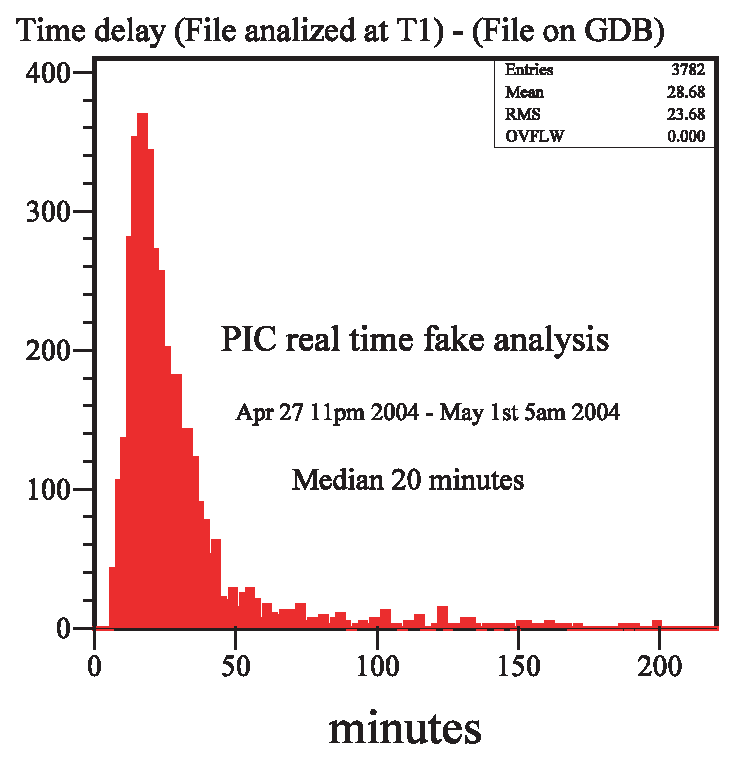
\includegraphics[width=10cm]{PIC-RTA.eps}
\label{fig:PIC-RTA}
\caption{During the last four days of DC04 PIC were able to implement a real% time analysis system based on CNAF's system. Turnaround time for analysis at  PIC was much shorter and more consistent than CNAF at a median of 20 minutes.}
\end{figure} 

Transfer rates varied greatly, and are treated in more detail below. Generally however, transfer rates at the start of DC04 were low- individual transfers reached maybe a MBps, with aggregate rates pushing 10MBps. These low transfer rates were due to the small size of files being pushed through the system- an example of poor initial coupling between the data source and the distribution system. Fortunately this poor coupling was improved to some extent by the implementation of a "merging" step (detailed below) which added files to one of a series of queues which expired and were written after either a certain aggregate size or time limit was reached. File sizes were typically ~500k median at the start of DC04.

(TODO: table of filesizes).

Agent uptime was not monitored directly, and is difficult to estimate. In many cases, for example, agents would not publish themselves as "available" if they could not complete any file transfers- as happened for example several times when the load on Castor was high. Interpretation of information about agent uptime is therefore difficult to interpret from DC04 logs. This is an area for improvement in future versions of the distribution system.

Due to bugs in the reconstruction code large numbers of files were deemed of limited use for analysis. It was decided that these files should be marked as bad, and effectively removed from distribution. To do this a new state- or rather set of states- indexed 90 and above was introduced. As agents weren't looking for files in those states, the files were never transferred. The system was therefore flexible enough to meet new requirements during development.

Coordination and management of people and agents proved highly inefficient, and it became clear that global mechanisms for suspending, restarting and monitoring agents needed to be deployed in future versions. During DC04, almost all system shutdown/restarts required an email sent to each operator, with the action only taken when all replies were received.

\subsection{The TMDB}
In contrast to other databases used, the TMDB proved to be remarkably stable, only experiencing a critical problem when log entries exceeded the initial tablespace allocated.

Development of the TMDB continued throughout DC04 as new use cases were discovered. The management of changes to the databases provided useful experience for the future. Most changes were easily accomodated thanks to a carefully designed database schema (for example, the addition of new agents was handled gracefully) (fig. \ref{fig:schema}).

\begin{figure}[tbp]
\centering
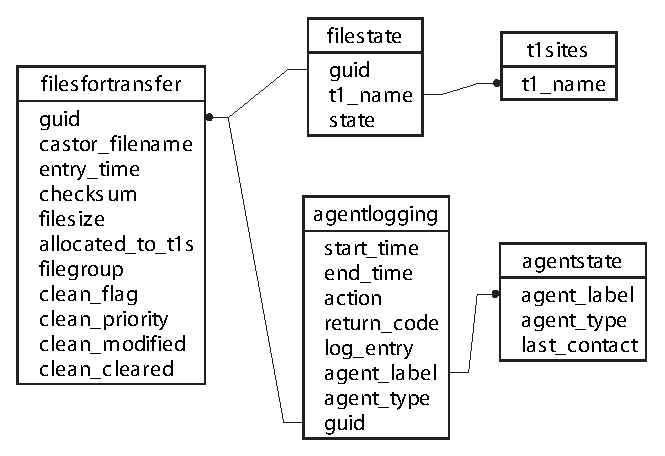
\includegraphics{v1_tmdb.eps}
\label{fig:schema}
\caption{The Transfer Management Database schema deployed during DC04.}
\end{figure} 

Some changes- notably the addition of some forms of metadata to the list of files for transfer- caused significant slow down in access. During DC04 it became apparent that some specific metadata- an entry denoting the filegroup, and some indication of cleaning priority- was required. Adding this new metadata was seen as a "one off", and was implemented as new fields in an existing table. At that stage, however, the TMDB had several hundred thousand files registered in it. The addition of new fields and entries to the database took many hours, and impaired access for the agents.

Future versions of the TMDB will require that metadata be stored in a separate table referencing filefortransfer.guid, thus avoiding this problem.

The discussion of which metadata to add to the database- from LFNs through replica to application metadata- continued throughout DC04. Addition of metadata to the TMDB was vigorously opposed to avoid it being seen as a permanent repository of metadata (in principle all information in the TMDB is transient). It became apparent that the ability to add metadata to replica entries- even changing the schema of metadata, or having a varying schema for each replica- was essential, especially during development.

\subsection{LCG Local Replica Catalogue (LRC)}
Good point was that it was used as a file and metadata catalogue for three
different distribution spaces, a use case not explicitly considered.

The LRC at CERN (somewhat ironically) provided a global file catalogue service for the main transfer components of DC04. It was found to be a critical bottleneck early in the challenge, and a significant amount of effort was expended in developing it so that performance was brought close to requirements. Even at the end of DC04 however it was still not ebing used generally- POOL XML catalogues were transferred alongside the data, and analysis either used these directly, or accessed the information via a local MySQL POOL catalogue if uploaded upon reacihng the destniation.

In general inserting information into the LRC was slow. Looking up file information by GUID met performance requirements, but queries, including queries by GUID, took a long time. Throughout DC04 discussions on performance were held with the catalogue developers, and as a result a new optimized version was released just after DC04.

TODO: This desperately needs some numbers for comparison! 

\subsection{Dropbox agents}
+ Performed well, typically 0.01s per drop (O(10) files).

+ Found needed bulk access to POOL RLS...

+ Numbers from Lassi.

\subsection{SRM chain}
The SRM distribution chain comprised an SRM Export Buffer at CERN providing access to a dCache disk pool, and an SRM import buffer at FNAL providing access to Enstore, again via dCache. 

At the T0, the SRM export buffer handled staging of files from Castor to dCache disk pool, where they were pinned until transferred.

The transfer agent copied files from the export buffer to the T1 import buffer by initiating a third aprty SRM transaction to receive a TURL from the export buffer, then using gridFTP to make the transfer.

The SRM chain provides the model by which future versions of the distribution system are intended to work, when sufficient components are available.

Initially problems were seen with repeated authentications: the agents were developed so that multiple streams, with multiple files in each stream, could be used to transfer files, reducing the number of authentications required. Transfer rates of over 10 MBps could be sustained for long periods (fig. \ref{fig:FNAL-network}).

\begin{figure}[tbp]
\centering
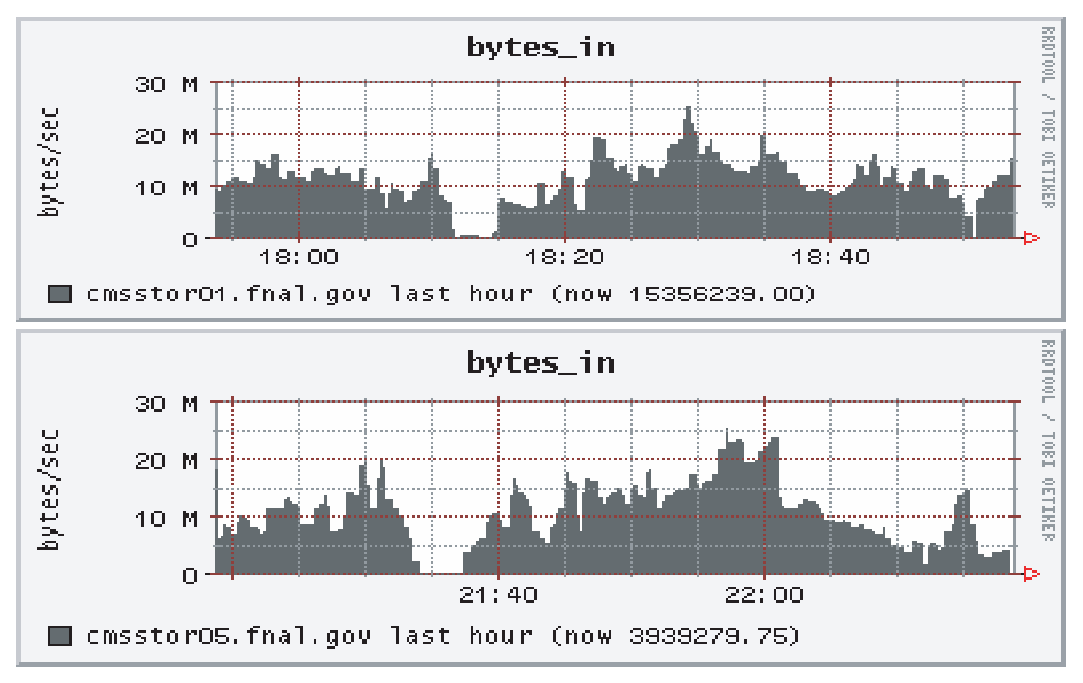
\includegraphics[width=10cm]{FNAL-network.eps}
\label{fig:FNAL-network}
\caption{The SRM chain was able to sustain transfer rates of more than 10 MBps into FNAL for long periods.}
\end{figure} 

In contrast to other techniques, the use of SRM eased agent development with features like automatic directory creation, file migration and staging, and automatic failure recovery.

However, during DC04 it proved difficult to install monitoring technology, which meant that hardware failures had to be identified by a human operator, and restarts handled manually. In common with other distribution chains the SRM chain had difficulties with the large number of small files, which necessitated an increase ni the number of tapes available and the deployment of a larger namespace service.

FNAL also deployed a MySQL POOL catalogue to enable access to the transferred data in the US; they found its performance more than adequate for the task. Initially the publishing of entries from the RLS to the FNAL POOL catalogue proved difficult, with the RLS queries taking a long time (see above). Close work between agent developers at CERN and FNAL brought about a 100-fold increase in performance.

All data access at FNAL was attempted through dCache via a ROOT plugin- so that COBRA based applciations could trivially access teh data. Read performance was shown to be "dramatically increased"- however, opening files became a dominant bottleneck, exacerbated by the large number of small files. The software environment consisted of access to applications over AFS at CERN, which proved quite stable.

Access to the transferred data was found to be logistically difficult: as the files ina  dataset were reconstructed at a range of times through DC04, they were stored on a large number of tapes. Making data available for analysis therefore meant a large number of tape stages.

Data was also transferred to UFL and Caltech T2s toward the end of the challenge. UFL was able to use the same software environment as the T1 to analyse data so transferred.

\subsection{SRB chain}
The performance of the SRB chain was severely hampered by technical issues:
first with availability of the MCat metadata catalogue, hosted at RAL, and
secondly with a small number of bugs in SRB client and server, and Oracle
Linux implementations. Experience with the SRB chain has highlighted the vital importance of production-quality service and support at the T1s, especially if they are to be responsible for mission-critical services during experiment running.

Within SRB version 2 the MCat, or metadata catalogue, represents a single point of failure. All user authentications, replica and metadata lookups are undertaken using this single service (it should be noted that this is not true in version 3 of SRB). 

However, SRB had been used successfully by CMS production for a year beforehand. In addition, LCG-2 resources were not available at several T1s. More critically still, for RAL and IN2P3 SRB represented the only mechanism available for placing files in mass storage.

Unfortunately during DC04 there came a serious break in service quality as staff at RAL left and replacements were sought, and then brought up to speed. As a result the MCat suffered serious problems on 22 of 56 days. Problems ranged from slight loss of performance (lengthy directory query times) to severe loss of performance (transactions taking so long that transfer agents had no choice but to continually time out) and unannounced reboots, geographical shifts of the database service and core dumps.

The SRB chain comprised an export buffer at the T0 and import buffers at RAL, IN2P3 and Karlsruhe T1s. Files were copied from Castor onto the export buffer, where they were injected (Sput) into SRB space. An application developed in the UK (GMCat) linked the name spaces of SRB and the other chains by publishing SRB replica information into the LRC at CERN periodically. Performance...

Even with administration problems, transfers to IN2P3 reached 10 MBps over a period of hours, although typically they averaged only 30 Mbps over a whole day. The SRB chain was not able to take part in a large filesize stress test at the end of DC04; these transfer rates are due to small file sizes, and thus compare favourably with other chains.



\subsection{LCG chain}
The LCG components required for distribution were the LRC at CERN, the dedicated information index (bdII), LCG-2 VO tools, a GridICE node at CNAF, Castor SEs at CNAF and PIC and "classic" disk SEs at CERN, CNAF, PIC, Legnaro and Taiwan.

At the start of DC04, the LCG chain had no Export Buffer from which to export data. A temporary storage element (SE) was deployed at CERN on March 3rd for testing. Ten days later a "classic" (e.g. disk based) LCG SE was deployed, and was joined by two other nodes several days later. This deployment represents intense effort by CERN IT/EIS and was critical in getting the LCG chain moving data.

The SE was managed as a distribution buffer by an EB agent, at first making third party transfers before being hosted by the SE node for reasons of efficiency.

Files from the SE EB were drained down to Castor SE buffers at CNAF and PIC T1s, then replicated to disk-SEs to grant data access for ``fake-analysis''. Throughout DC04 the SE agent and the PIC and CNAF T1 agents were all able to match pace with the generation of files at the T0 (fig. \ref{fig:PIC-FT}).

\begin{figure}[tbp]
\centering
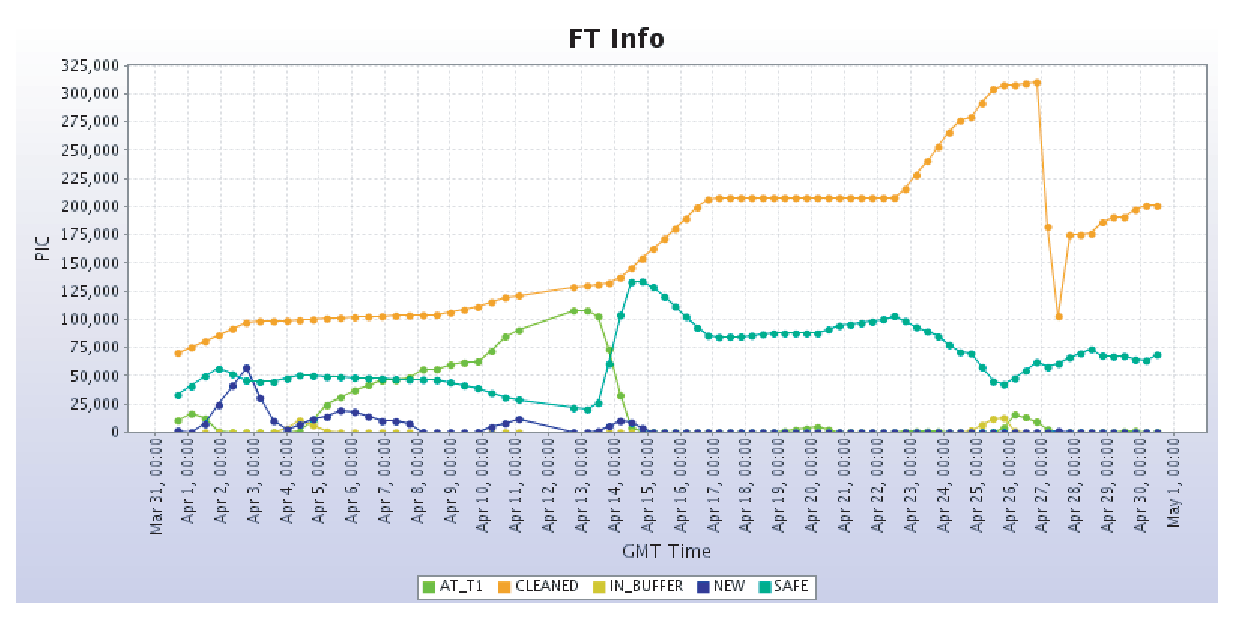
\includegraphics[width=10cm]{PIC-FT.eps}
\label{fig:PIC-FT}
\caption{Throughout DC04 the number of files apparently at the T0 and on the SE (classed as NEW or IN\_BUFFER) was negligible for PIC and CNAF (the diagram here is for PIC, but is equally applicable to CNAF), suggesting that the SE and T1 agents were able to keep up with the rate of generation of files at the T0. }
\end{figure} 

At the start of DC04 both used the Java RM API to make transfers and catalogue lookups/registrations. This was found to be inefficient. Interestingly, the T1s chose subtly different methods to transfer from the T0 after moving away from the Java API.

CNAF chose to use the EDG RM C++ API with some very limited use of the LRC C++ API. Use of the RM API meant that their transfers and catalogue registrations were integral operations, and therefore more fully transactional. PIC chose to use globus-url-copy and the LRC C++ API to register replicas. In principle recovering from failed transfers was more costly for PIC: this however should be weighed against CNAF's use of the slower RM API.

Subtle variations in approach aside, transfer rates from the SE EB could be sustained at over 2 MBps, peaking at 16 MBps (fig. \ref{fig:SE-EB-network}), with transfer rates into CNAF and PIC reaching a sustained 30 MBps for hours during a large-filesize stress test at the end of DC04 (fig's. \ref{fig:PIC-stress}, \ref{fig:CNAF-stress}). Internal monitoring at CNAF revealed a bottleneck on site, with an internal link to the SE operating at over 80\% capacity during the final stress test.

\begin{figure}[tbp]
\centering
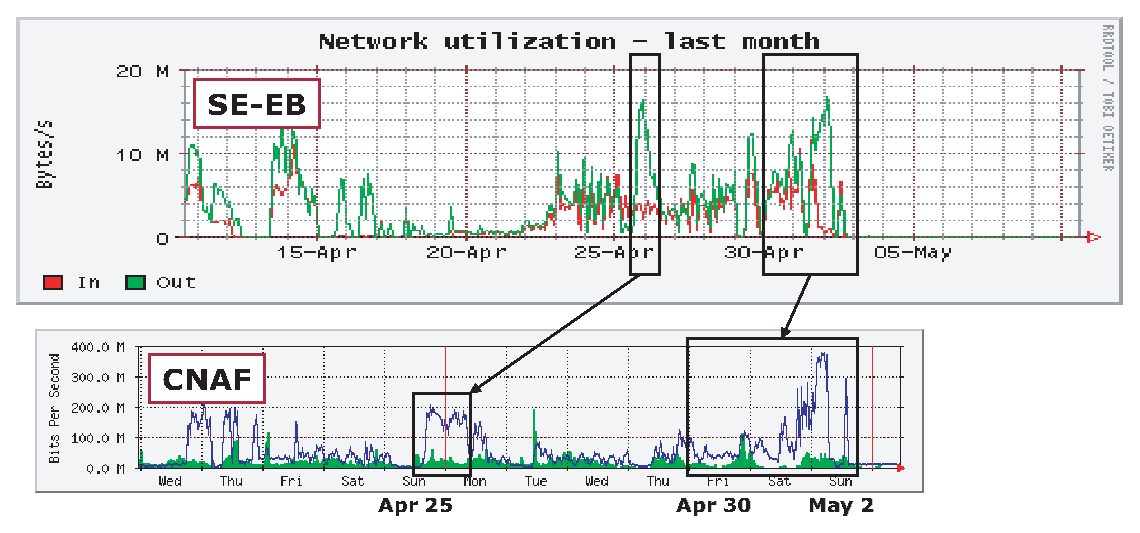
\includegraphics[width=15cm]{SE-EB-network.eps}
\label{fig:SE-EB-network}
\caption{Transfer rates out of the SE EB could be sustained at over 2 MBps toward the end of DC04, and peaked at 16MBps.}
\end{figure}

\begin{figure}[tbp]
\centering
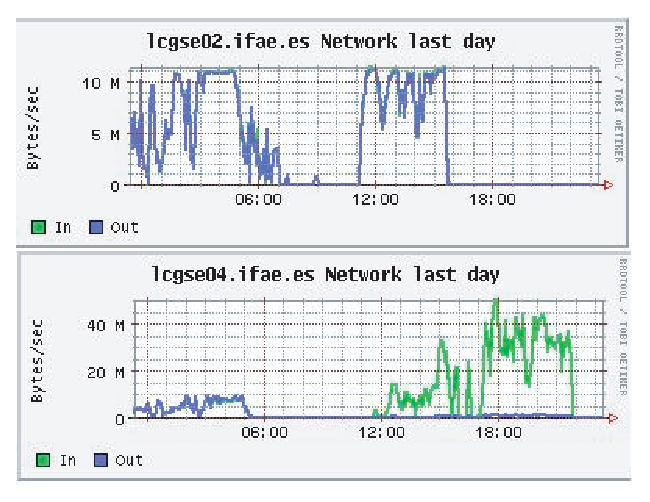
\includegraphics[width=10cm]{PIC-stress.eps}
\label{fig:PIC-stress}
\caption{During a large filesize stress test at the end of DC04, files of 600MB and larger were put into distribution. PIC sustained transfer rates of 30 MBps for 6 hours.}
\end{figure} 

\begin{figure}[tbp]
\centering
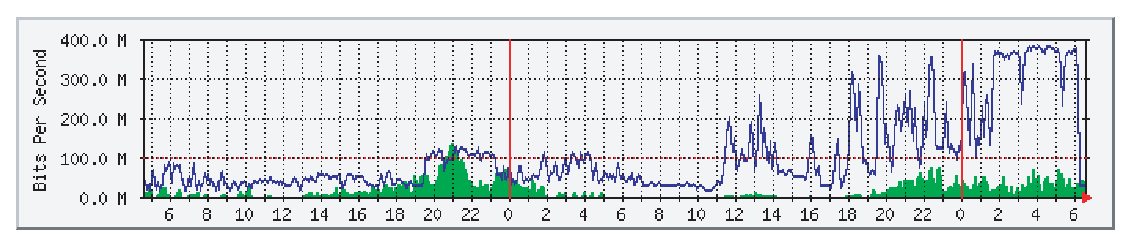
\includegraphics[width=10cm]{CNAF-stress.eps}
\label{fig:CNAF-stress}
\caption{During a large filesize stress test at the end of DC04 (the period from 0 at the right of the plot), files of 600MB and larger were put into distribution. CNAF sustained transfer rates of 40 MBps for 5 hours.}
\end{figure} 

At CNAF issues with the Castor tape stager were found to be due to the high number of entries in its database (a consequence of the small file size). In general tape performance was slow due to inefficient utilization, meaning a delay in psoting files as being ``safe''. CNAF have since been working on an import buffer and related agents to group files more reasonably for their tape system on arrival.

In contrast PIC experienced no problems with their Castor tape.

PIC and CNAF were also able to distribute data on to T2s (X and Legnaro respectively) for analysis. To manage these further transfers, as well as real-time analysis, they effetively created a new set of distribution chains using a MySQL TMDB for collaboration information.

%\subsection{Real-time analysis agents}
%Real-time analysis- analysis of data as it arrived at the T1- was successfully attempted at CNAF, PIC, FNAL and IN2P3, with varying performance. 

%At CNAF, the T1 transfer agent notified a real-time analysis agent when new files were available for analysis. The eal-time analysis agent submitted analysis jobs on the new data using BOSS through LCG-2 RBs at CERN and CNAF, with the jobs being directed to CEs at CNAF or Legnaro. 

%15000 jobs were submitted in this way over the last two weeks of DC04. The minimum period between the files appearing in distribution and being analysed was 10 minutes- but with a large number of ``outliers''. 

%The outlying longer times were attributed to: the fact that datasets were completed over a relatively long length of time at CERN; Castor problems at CNAF reduced replication efficiency; analysis agents were actively developed during this period and were therefore not up all the time; and occasionally zipped metadata arrived late compared to the related dataset, delaying analysis.

%An analysis of the performance of a single job showed that the ORCA execution time was 25 minutes. For comparison, the time to stage files was just short of 3 minutes, and the overhead of submission to the Grid was only 2 minutes. Efficiency of submission to the grid was over 95\% (fig. \ref{fig:CNAF-RTA}).

%Significantly, the maximum rate of job submission was 194 jobs per hour- which corresponds to 26 Hz (or events per second), the target rate for DC04.

%\begin{figure}[tbp]
%\centering
%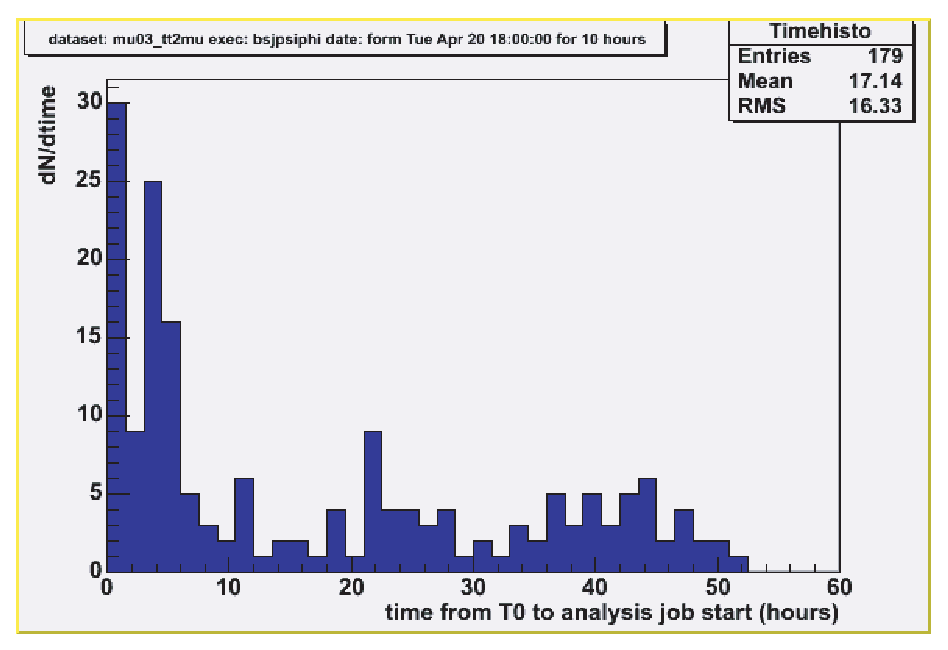
\includegraphics[width=10cm]{CNAF-RTA.eps}
%\label{fig:CNAF-RTA}
%\caption{During the last two weeks of DC04 CNAF was able to analyse data in %real time (or syncronously with the production of data). The minimum period between the appearance of files in distribution was 10 minutes. There is however a significant population of longer periods shown here, which were attributable to a number of issues like ongoing development of the analysis agents. It should be noted that CNAF was "in the front line" with real time analysis, and were the first to develop and deploy the system described here.}
%\end{figure} 

%Over the last four days of DC04 PIC was able to adapt the INFN real time analysis agents for their local environment, which included a private (dedicated) LCG-2 Resource Broker and Grid Information System. Job submission was not coordinated through BOSS due to lack of time and the necessity of sending large executables through the sandbox. Instead the agents communicated through a local MySQL database, and by making drops of XML catalogues for each other.

%The period between files appearing in distribution and undergoing analysis was noticeably shorter and more consistent at PIC: the median period was only 20 minutes, with 13 minutes median transfer time (fig. \ref{fig:PIC-RTA}).

%\begin{figure}[tbp]
%\centering
%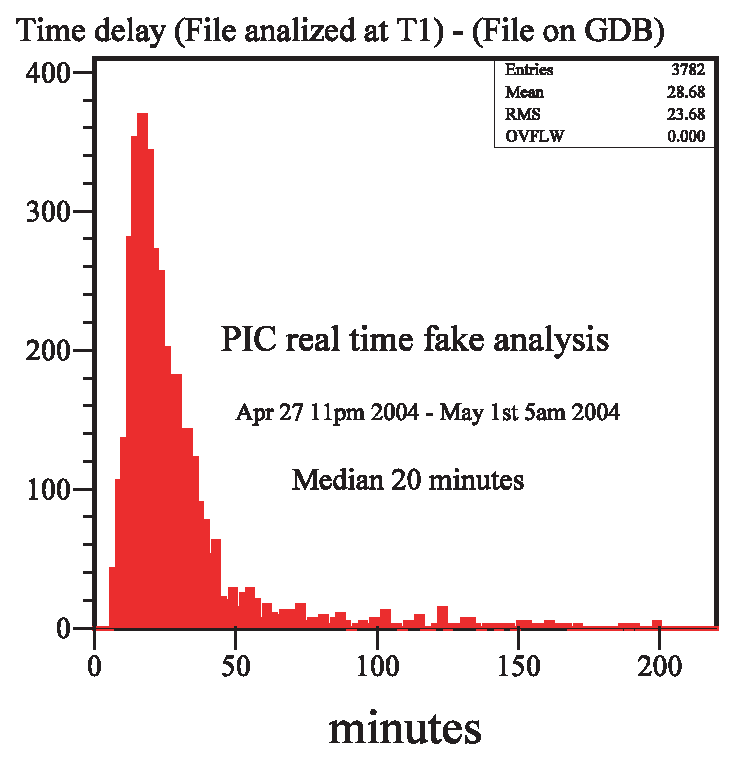
\includegraphics[width=10cm]{PIC-RTA.eps}
%\label{fig:PIC-RTA}
%\caption{During the last four days of DC04 PIC were able to implement a real% time analysis system based on CNAF's system. Turnaround time for analysis at PIC was much shorter and more consistent than CNAF at a median of 20 minutes.}
%\end{figure} 

%TODO: Specific reasons why PIC turnaround time was shorter and more consistent that CNAF.

%TODO: At Fermilab a mean period of 252 minutes elapsed between availability and analysis ... over the Grid, of what type...? (fig. \ref{fig:FNAL-RTA}).

%\begin{figure}[tbp]
%\centering
%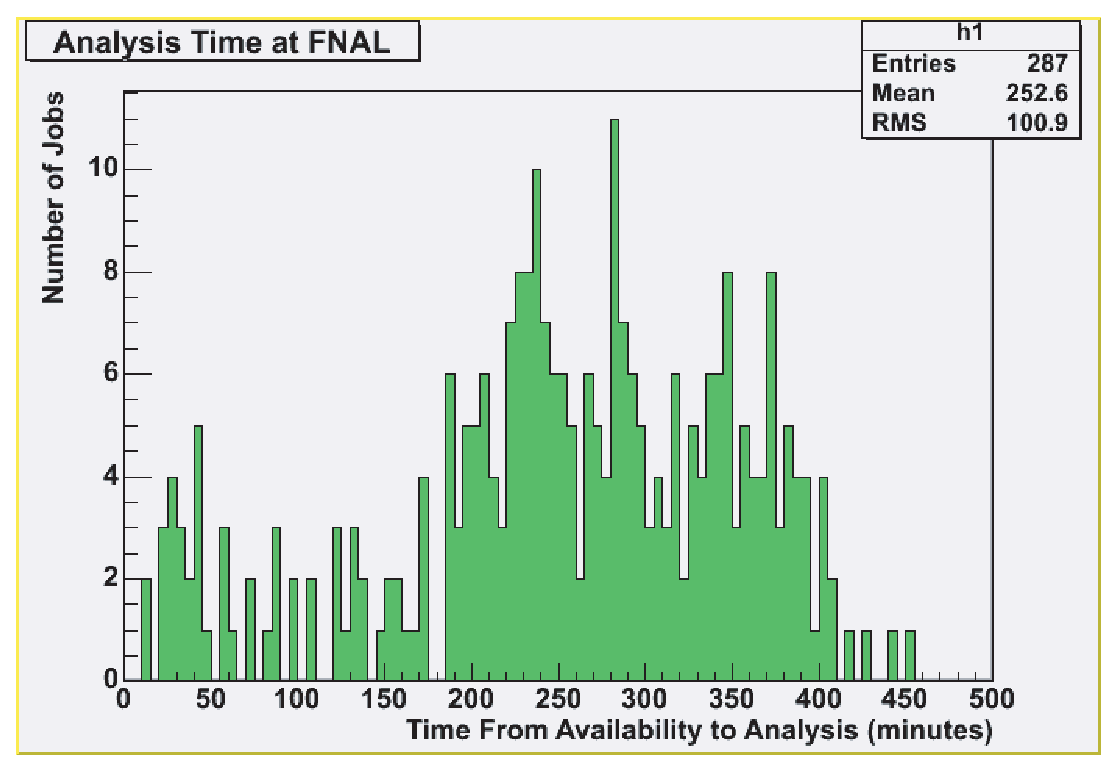
\includegraphics[width=10cm]{FNAL-RTA.eps}
%\label{fig:FNAL-RTA}
%\caption{A caption here :)}
%\end{figure} 


\section{Conclusions and future plans}
Sources of throttling: access to tape/stage, catalogues, tmdb(?), intermediate links (no control over these?), buffer read/write, tape migration...

Gap in middleware: developers have implemented APIs. They have also developed command line tools which are good as examples but suffer from impaired performance when used in a large scale system. From our point of view the amount of "grid itegration" work to is alrger than expected: many expected the middleware developers to develop tools rather than APIs.

A general remark about "more warning and planning so that operational issues could be anticipated".

Data sources and distribution need to be coupled properly- for example, reconstruction produced many small files, whereas distribution requires large files to function efficiently. Impedance mismatches?

Most "big pushes" planned over the weekend! Not the best of ideas? Could it be done any other way?

Management of agents in a global sense, and notification of local supervisors needs to be dramatically improved in future versions of the system, as email does not provide an efficient and reliable mechanism for coordinating agent shutdown and restart, and other global system actions.

IT was shown that it is possible to analyse data as it arrives, with only a 20 minute period elapsing between the file being made available for distribution and it being used in analysis. This turnaround time gives us confidence that future versions will be able to handle this sort of analysis consistently and for sustained periods. The variability in eprformance between deifferent deployments of the real-time analysis agents and structure however shows that there is some exploraty work to be done to determine the best practice for deployment and use.

The distribution system/ agents require easy access to metadata, both dedicated distribution metadata and more experiment specific emtadata. The mechanism for handling this was poorly developed for DC04, and needs to be improved for future versions. However, it is important that people remember that the TMDB is not a permanent repository of metadata, as the information it contains will probably be deleted once the files are no longer in transit.

Logging of low level metrics- file transfer rates, etc- was handled very well by a number of tools- MonaLISA, GridICE, Lemon among them. Logging of higher level distribution component metrics however was not so well developed. Toward the end of DC04 the number fo files in each state was monitored using MonaLISA, but only for a predefined set of states (e.g. the total set of states was not dynamically determined). In the future this monitoring needs to be extended to cover agent uptime, transition of files through states, files handled per agent per second and no doubt others.

Log entries should not be made in the TMDB- instead they should be handled locally by a tool such as netlogger- note that remote access to these logs on demand is still necessary; it should be pssible to query the log repository remotely.

\bibliographystyle{plain}
\bibliography{dc04-post-mortem}





\appendix{The Transfer Management Database and the distribution system}
\section{Building the system}
The goal of the distribution system was to consistently store data from the Tier 0 in a storage media that is considered safe (e.g. MSS) at a number of Tier 1 sites. The structure described here used a common database (TMDB) that was available for read/write by all agents.

Reco data was placed in a "general distribution buffer" (maybe flat file space) at the Tier 0. Beyond these requirements each data distribution system
(e.g. LCG, GridFTP, SRB) will have its own requirements of buffer/staging space at T0 and T1s, although each method should meet the basic requirement of publishing file state information in the common database: that an entry of SAFE is made for each file when it has been safely stored in mass storage at each Tier 1 to which it is assigned.

\subsection{The Transfer Management Database (TMDB)}
The Transfer Management Database provided a space in which transfer agents communicated information. This information was principally file state metadata. The file state was used to determine the availability of files at  different stages of the distribution, and ultimately its safe storage on tape at a number of allocated T1s.

\subsubsection{Users, servers}
The tablespaces DATA01 and INDX01 existed on pdb01.cern.ch and devdb9.cern.ch. The former had 2GB on each tablespace, the latter only 100 MB, to be used for testing. The following users could access the database:

\begin{tabular}[tbp]{|l|l|}
\hline User & Description
\\ \hline CMS\_TRANSFERMGMT & With 2GB quota on both of the DATA01 and INDX01 dedicated tablespaces.
\\ CMS\_TRANSFERMGMT\_WRITER & Limited read and write permissions.
\\ CMS\_TRANSFERMGMT\_READER & Read only permissions.
\\ \hline
\end{tabular}

\subsection{Schema}

TODO: See schema diagram at end of doc

\subsubsection{t1sites}
\begin{tabular}[tbp]{|c|c|c|c|}
\hline \multicolumn{4}{|c|}{t1sites}
\\ \hline field & type & constraints & index
\\ \hline t1\_name	& char(20) & primary key &
\\ \hline
\end{tabular}

{\bf t1sites} held the core list of T1s, to be used as a Foreign Key constraint on other tables. Sites in action at the start of DC04 were labelled as

\begin{tabular}[tbp]{|c|c|} 
\hline T1 & t1\_name
\\ \hline RAL & RAL		
\\ FNAL & FNAL
\\ IN2P3 & IN2P3
\\ PIC & PIC
\\ FZK & FZK
\\ \hline
\end{tabular}

�New� T1s could be added to this list if they contribute resources or if existing T1s change distribution scheme. This did not occur during DC04.

\subsubsection{filesfortransfer}
\begin{tabular}[tbp]{|c|c|c|c|}
\hline \multicolumn{4}{|c|}{filesfortransfer}
\\ \hline field & type & constraints & index
\\ \hline guid		&		char(36) &		primary key &
\\ castor\_filename	&	char(250) & &
\\ entry\_time		&	int & &
\\ checksum		&	int & &
\\ allocated\_to\_t1s	& char(1) & & x
\\ \hline
\end{tabular}

Guid indicates the unique identifier for a replica, and is of defined length. castor\_filename was the location of the file in Castor. The guid-Castor mapping will already be present in the LRC: it was also placed here to avoid extra LRC lookups. entry\_time was a unix timestamp (i.e. seconds since epoch start) of first entry into the distribution system. checksum was a normal unix checksum (generated with cksum). allocated\_to\_t1s indicated the state of the file (0 == true, !0 == false). false indicated files newly placed by Reco, true indicated that the configuration agent had allocated it to a number of T1s.

\subsubsection{filestate}
\begin{tabular}[tbp]{|c|c|c|c|}
\hline \multicolumn{4}{|c|}{filestate}
\\ \hline field & type & constraints & index
\\ \hline guid		&		char(36) &		primary key &
\\ t1\_name			& char(20)	& foreign primary &
\\ state			& int	& & x
\\ \hline
\end{tabular}

Guid again stored a unique file identifier, forming a primary key with t1\_name (a foreign key taken from t1sites). state indicated the current state of the propagation of the file. The following states were thought necessary: NEW, EB REALLOCATED, T1 REALLOCATED, IN BUFFER, AT T1, SAFE, CLEANED. During DC04, further states were added- some T1 specific, and some BAD states used for global management. Not all states were required, however- as failover was not tested in production, states EB and T1 REALLOCATED were not used.

The states were enumerated-

\begin{tabular}[tbp]{|c|c|} 
\hline index & state
\\ \hline 1	& NEW
\\ 2	& EB REALLOCATED
\\ 3	& T1 REALLOCATED
\\ 4	& IN BUFFER
\\ 5	& AT T1
\\ 6	& SAFE
\\ 7	& CLEANED
\\ 8+	& T1 specific
\\ \hline
\end{tabular}

TODO: there were more states at the end than this!

as agents were the most frequent accessors of this information, and human operators accessed it via some front end which could interpret the state for them.

\subsubsection{agentstate}
\begin{tabular}[tbp]{|c|c|c|c|}
\hline \multicolumn{4}{|c|}{agentstate}
\\ \hline field & type & constraints & index
\\ \hline agent\_label		& char(20)	&	primary key &
\\ last\_contact	& 	int & &
\\ \hline
\end{tabular}

agent\_label was a text string that uniquely identified a distribution component-

\begin{tabular}[tbp]{|c|c|} 
\hline component & label
\\ \hline LCG SRM EB agent	& SE\_EB	
\\ GRID3 SRM EB agent	& SRM\_EB\_DCACHE
\\ SRB EB agent		& SRB\_EB
\\ RAL transfer agent	& RAL
\\ FNAL transfer agent	& FNAL
\\ IN2P3 trans. agent	& IN2P3
\\ PIC transfer agent	& PIC
\\ CERN transfer agent	& CERN
\\ FZK transfer agent	& FZK
\\ \hline
\end{tabular}

TODO: There were more agents than this!

and was used as a foreign key for other tables. Agents were required to periodically make contact with the database by updating last\_contact. Any agent failing to update over the predefined period was considered to be unavailable

\subsubsection{agentlogging}
\begin{tabular}[tbp]{|c|c|c|c|}
\hline \multicolumn{4}{|c|}{agentlogging}
\\ \hline field & type & constraints & index
\\ \hline agent\_label		& char(20)	 & foreign &
\\ guid				& char(36)	 & foreign &
\\ start			& int & &
\\ end				& int & &
\\ action			& char(20) & &
\\ return\_code	 &	int & &
\\ log\_entry			& char(250) & &
\\ \hline
\end{tabular}

agent\_label was a unique agent label as described above; similarly, guid uniquely defined a file replica. start and end indicate the period over which the entry was relevant (i.e. for file transfer log entries). action contained one of a number of globally defined quick search entries (these were open for discussion/additions, but should definitely be globally agreed).

TRANSFER
Single entry per file transfer.

START
When agent starts.

FOUND
When agent checks transfer management tables and finds file entries to deal with (used during normal operations and recovery phase).

LEASED
When agent updates the agent state database.

FAIL
When agent needs to shut down (e.g. buffer has filled up, etc).

return\_code was used to store the return code of the operation that the log entry refers to. log\_entry provided a means to supply more descriptive entries if necessary.
 
\end{document}
